\chapter{Introduction to Lightning Network}

\label{Chapter05IntroLightning}

In this Chapter, we present an introduction to the second layer (L2) blockchain protocols and in particular the Lightning network for Bitcoin.

\section{Introduction to blockchain scaling}

Bitcoin was designed to avoid trusted third parties.
If there is no designated servers to validate transactions, then all users must do this, or at least be able to.
This design choice imposes severe restrictions on transaction throughput, with a theoretical maximum of tens of transactions per second~\cite{Croman2016}.
Even if executing Bitcoin scripts is relatively cheap in terms of computation, users with consumer hardware should be able to keep up with the network in real time.
Otherwise, if the inflow of new transactions per unit time is higher than a user's device can validate, the user would have to trust a third party with more powerful hardware to tell whether transactions are valid.

Accommodating the increased demand for transactions requires protocol update.
Let us consider ways in which open blockchain protocols such as Bitcoin can be updated.

\subsection{Soft forks and hard forks}
Blockchain networks have a unique property compared to other software in how they are updated.
In a decentralized network, there is not master switch that can force users to update.
Instead, Bitcoin's updates must achieve consensus among the majority of interested parties: full node operators, miners, businesses, wallet developers, and so on.
Moreover, the development philosophy of Bitcoin strictly opposes breaking changes.
The rationale is that all coins must be spendable under the same conditions as at the time they had been locked.
For instance, even is a more efficient signature algorithm is implemented in Bitcoin, it must be an addition to the old one, not a replacement.

The non-breaking type of update is referred to as a \textit{soft fork}.
In a soft fork, the rules of the protocol become more strict.
Therefore, a non-updated node would still perceive blocks created under the new rules as valid, though it may not understand all of the new semantics.
In practice, soft forks are often implemented by enhancing one of the \texttt{OP_NOP} opcodes with the new semantics.

A breaking updated is referred to as a \textit{hard fork}.
A hard fork broadens the set of valid blocks.
This means that a block created under the new rules may be invalid from the viewpoint of old nodes.
Increasing the block size is an example of such change: if the limit is raised (like in Bitcoin~Cash), an 7~MB block, which fits under the new limit, is rejected by old node.

\subsection{Bitcoin block size debate}

This restriction is manifested in Bitcoin's code with the \textit{block size limit}.
In 2010, Satoshi Nakamoto introduced a 1~MB limit on the block size~\cite{Nakamoto2010}.
With the growth of the Bitcoin ecosystem, dismantling this restriction has become less and less likely due to the disruption it would cause.

A subset of the Bitcoin community viewed the 1~MB restriction as a limiting factor for Bitcoin's adoption in retail.
To make Bitcoin a common means of payment worldwide, one would argue, the system would have to handle more transactions than under the 1~MB limit.
Otherwise the fees would rise, and using Bitcoin for small purchases would become uneconomical.
A counterargument to this was that raising the block size limit, apart from causing disruption, would cut off less powerful hardware from validating transactions, hindering the ability of users to independently validate transactions -- the key property of the system.

This contradiction lead to a conflict within the Bitcoin community, culminating in 2017 with the introduction of Bitcoin~Cash and the activation of \textit{segregated witness} (SegWit).
Bitcoin~Cash is a cryptocurrency born as a hard fork of Bitcoin with the block size raised to 8~MB.
Bitcoin (as defined by the Bitcoin~Core codebase) introduced another method of increasing throughput -- segregated witness (SegWit).
This thesis focuses on the scaling approach taken by Bitcoin~Core\footnote{While Bitcoin~Cash proponents tend to refer to the version of Bitcoin with SegWit as Bitcoin~Core to stress the proposition that both forks have equal rights to inherit the name "Bitcoin", we'll refer to the Bitcon~Core implementation as Bitcoin.}.

\subsection{Segregated witness}

SegWit was an important milestone in the evolution of Bitcoin.
This protocol change, as the name suggests, \textit{segregated} the \textit{witness} (that is, the transaction signatures) from the part of the blockchain data used to calculate transaction hashes).
The block size has been replaced by block \textit{weight} -- a synthetic metric which assigns different parts of a transaction different weights when counting towards the total weight of a block.
The old block \textit{size} limit has been internally converted to block \textit{weight} limit.
This resulted in the actual block size limit being increased to 4~MB without a hard fork.

More importantly for our work, SegWit solved the \textit{transaction malleability} issue.
This has been a fundamental roadblock that has been holding back the development of layer-two protocols.
Due to the qualities of ECDSA signatures and their implementation in OpenSSL library used in Bitcoin, and also to properties of Bitcoin scripts, it was possible for an attacker, given a signed transaction, to modify it and this change its hash without changing its semantics.

In the context of L2 protocols, this is a critical drawback.
L2 inherits its security properties from L1, assuming that parties can check whether an event of interest has happened on L1.
For instance, to prevent cheating, the protocol must ensure that Alice can understand by looking at the blockchain whether Bob is attempting to cheat (for instance, broadcast an old channel state), and vice versa.
With transaction malleability, the attacker could replace an unconfirmed transaction with another transaction with the same semantics but different hash.
This makes "watching" the blockchain for relevant messages hard, if not impossible.

With SegWit, transaction signature (witness) no longer affects its hash.
Therefore, a hash reflects only the transaction \textit{semantics}, omitting the \textit{proof} of its validity.
This allows LN parties to watch the blockchain for specific transaction hashes and be sure that the \textit{behavior} they are interested in cannot be performed on layer-one in any other way.
We will describe the mechanics of the Lightning protocol in detail later in this Chapter.


\subsection{L2 protocols in Ethereum and other blockchains}

While this part of the thesis focuses on Bitcoin's L2 protocols and LN in particular, payment channels are only one type of layer-two protocols.
For completeness let us mention some of the related developments in the Ethereum ecosystem.

Ethereum is \textit{the} other major open blockchain alongside Bitcoin\footnote{It is second in the market capitalization and first in the number of transactions~\cite{Coinmetrics}. Due to the differences in transaction mechanics and semantics, meaningfully comparing the metrics of these two major blockchain networks is a separate research question.}.
Ethereum makes many architectural decisions differently from Bitcoin.
It incorporates a \textit{Turing-complete programming language}, supports \textit{zero-knowledge cryptography}, and is explicitly \textit{stateful}.
This complexity of the base protocol is reflected in a wider space of layer-two designs, which include refereed computation protocols (Arbitrum~\cite{Kalodner2018}, Truebit~\cite{Teutsch2017}), state channels (Sprites~\cite{Miller2019}, Perun~\cite{Dziembowski2017}), Plasma~\cite{Poon2017}, and rollups (optimistic~\cite{Floersch2019}, zk-rollups~\cite{Gluchowski2019}).


\section{Evolution of payment channels in Bitcoin}

Layer-two protocols allow blockchains to scale without modification to the base layer (\textit{off-chain scaling}).
In the context of Bitcoin, layer-two protocol usually implement the concept of \textit{payment channels}.
A payment channel allows its two participants to exchange transactions without broadcasting them to the blockchain.
Some of the security guarantees of L1 are preserved: conflicts can be resolved on layer-one.
We refer the reader to a comprehensive overview of off-chain approaches in~\cite{Gudgeon2019}.

Multiple ideas or implementations of Bitcoin channel for Bitcoin have been proposed.
To put our work on the Lightning Network in historical context, we now describe the evolution of layer-two protocols in Bitcoin following the outline in the Bitcoin wiki~\cite{BitcoinWikiChannels}.

\subsection{Transaction replacement with sequence numbers}

Satoshi Nakamoto proposed what was arguably the first protocol for re-negotiating a transaction without broadcasting it.
This mechanism takes advantage of two Bitcoin features: transaction sequence number (\texttt{nSequence}) and time lock (\texttt{nLockTime}).

Bitcoin initially implemented a mechanism for replacing unconfirmed transactions.
Each transaction has an \texttt{nSequence} field, which acts as a counter.
The protocol prescribed miners to give priority to transactions with higher sequence numbers (regardless of fees).
The time lock field (\texttt{nLockTime}) mandates a time before which a transaction cannot be confirmed in a block, expressed as a timestamp or a block height.
The transaction replacement protocol would prescribe the two parties to sign a series of transactions with an increasing sequence number and a timelock at some point in the future.
The final state would be confirmed after the timelock expires.

The major problem with this approach is that sequence numbers are not enforceable.
If the two parties disagree on which of the signed transaction should be confirmed on the blockchain, the miners are not forced to choose the one with a higher sequence number.
Miners do not get punished even if they deliberately confirm a transaction with a lower sequence number, possibly as a result of a collusion with one of the channel parties.
They even have a degree of plausible deniability: they may claim that they simply have not heard of the later transaction versions, which may happen without malicious intent due to P2P propagation delay.


\subsection{Unidirectional channels}

The first version of unidirectional channel, Spillman channels, introduced in 2013, is a modified implementation of the Nakamoto payment channels~\cite{Spillman2013}.
This protocol for micropayments has been implemented in BitcoinJ, a popular Java Bitcoin library~\cite{BitcoinJ}.

Spillman channel use what~\cite{Gudgeon2019} describes as \textit{revocation by incentive}.
Initially, the customer and the merchant lock coins into a multisignature output.
Additionally, they establish a time-locked refund transaction, which would allow the customer to withdraw all funds in case the merchant goes offline.
Then the client signs and sends to the server a transaction which distributed the coins from the funding transaction in a new proportion, allocating more funds to the merchant.
The merchant can either co-sign and broadcast it, thus closing the channel, or wait for the next transaction version.
Shortly before the timelock of the refund transaction expires, the merchant broadcasts the latest transactions, confirming the agreed upon balances.

This protocol has a number of drawbacks.
First, it is unidirectional: the customer can pay the merchant but not vice versa.
Second, the lifetime of a channels is limited by the timelock of the refund transactions.

Note that the protocol is not secure if transactions are malleable.
In particular, an adversary modifying the funding transaction without invalidating it would invalidate the refund transaction~\cite{Harding2016}.
After SegWit activation this is no longer the case, if the customer is using SegWit outputs.

A similar design of unidirectional payment channels takes advantage of \texttt{OP\_CHECKLOCKTIMEVERIFY} (CLTV) -- a new opcode added in 2015~\cite{Todd2014}, which allows to specify absolute timelocks on an output level (as opposed to transaction level for \texttt{nLockTime}).
This allows to implement Spillman channels without the malleability vulnerability.
\footnote{Note that CLTV was implemented in 2015, before SegWit (2017).}


\subsection{Replace-by-timelock and Duplex channels}

Relative timelocks allow for another channel protocol, supporting bidirectional payments.
Remember that the key problem in channel constructions is to invalidate old channel states.
While Nakamoto channels rely on unenforceable sequence numbers, Spillman's protocol leverages economic incentives.
It is most profitable for the receiver to broadcast the last transaction.
This restricts Spillman channels to unidirectional use case.

With timelocks, it is possible to implement bidirectional channels.
In a series of off-chain transactions, each transaction must be time-locked to a point closer to the present than the previous one by a safety margin.
The drawbacks of this construction are limited channel lifetime (determined by the timelock of the initial transaction) and the limited total number of potential updates (determined by the total channel lifetime and the safety margin between timelocks).

Duplex micropayment channels, proposed by Decker and Wattenhofer~\cite{Decker2015}, combine replace-by-timelock and replace-by-incentive to implement bidirectional channels as a pair of unidirectional channels.
The key concept of DMC is \textit{invalidation tree} -- a hierarchical transaction structure that allow for invalidation of old channel states.


\subsection{Poon-Dryja channels (Lightning)}

Lightning channel have been proposed by Poon and Dryja in~\cite{Poon2016}.
Lightning overcomes the limitations of previous channel designs.
LN channels are \textit{bidirectional} and have an \textit{unlimited lifetime}.

The key insight in Lightning is its \textit{revocation mechanism}.
The transactions reflecting channel states are constructed in such a way that each next update \textit{invalidates} the previous one.
Despite the fact that all intermediate states are valid Bitcoin transactions (and can be broadcast and confirmed on the blockchain), broadcasting any state except the latest one by one party allows the other party to withdraw \textit{all} funds from the channel, punishing the cheater.
We will describe the Lightning protocol in more detail later.


\subsubsection{Future of Lightning}

As of 2020,~LN is being used in production but is still under heavy development.
Some of the ideas to improve LN depend on modifications in the Bitcoin protocol, which usually take a long time to implement, test, and roll out.

\paragraph{Schnorr-Taproot}
As of early 2020, the Bitcoin community is waiting for the implementation and rollout of the \textit{Schnorr-Taproot} update.
This would allow for another type of signatures (Schnorr signatures in addition to ECDSA), which allow for arithmetic on signatures.

For Lightning Network, this allows for better privacy.
The current HTLC mechanism maintains atomicity of multi-path transfers by using the same payment hash along the whole route.
This breaks relationship anonymity: an attacker controlling two nodes along the route can trivially learn that the two channel updates are part of the same transaction.
To address this attack, new cryptographic constructions replacing HTLC have been proposed.
Atomic multi-hop locks (AMHL)~\cite{Malavolta2019} and Payment points~\cite{Kohen2019} allow for the same functionality as HTLC but with randomized payment secrets for every hop in the route.
These improvements can be implemented after Schnorr-Taproot is activated, which may happen in 2020.

\paragraph{eltoo}
An alternative payment channel proposal, eltoo, has been proposed by Decker, Russell, and Osuntokun~\cite{Decker2018}, as Lightning has been already established as a major Bitcoin scaling effort.
Eltoo proposes an arguably more efficient revocation mechanism, where intermediary transactions are linked to each other linearly (as opposed to all of them spending the same output of the funding transaction in the current LN), and only on channel closure the final transaction is "re-attached" to the funding transaction's output.
This requires a new \textit{signing flag} (\texttt{SIGHASH\_NOINPUT}~\cite{Decker2017}) not yet implemented.
\footnote{A signing flag specifies whether a signature commits to all or only some of a transaction's inputs. Allowing a transaction to \textit{not} commit to any input allows for "re-attaching" a signed transaction to a compatible output, which eltoo uses for channel state revocation.}
If \texttt{SIGHASH\_NOINPUT} is implemented, eltoo revocation mechanism can be used in LN or in a separate payment channel network.

\paragraph{Privacy-preserving channels}
A payment channel protocol called Bolt\footnote{Not to be confused with Basics of Lightning Technilogy (BOLT) -- the Lightning Network specification.} has also been proposed for a privacy-focused cryptocurrency Zcash~\cite{Green2017} and later modified for compatbility with Bitcoin-like blockchains (including Bitcoin itself) and renamed to zkChannels~\cite{Akinyele2020}.


\section{Lightning network overview}

The Lightning Network (LN) has emerged as the alternative to the scalability issue of Bitcoin with the highest adoption in practice~\cite{Cuen2019}.
%LN has experienced rapid growth since its launch in early 2018~, 
As of February~2020, LN facilitates the off-chain exchange of nearly $900$~BTC.
The principles of the LN can be used to improve the scalability of other cryptocurrencies. 
For instance, similar networks operate with Litecoin~\cite{1MLLitecoin} and Ethereum~\cite{RaidenWebsite}. 



\subsection{Nodes and channels}

Each \textit{LN node} is defined by an ECDSA private-public key pair.
A persistent \textit{node identifier} is derived from the hash of the public key. 
Additionally, the owner can assign a human-readable alias to their node.
Operations from a node are authorized with a digital signature created with the corresponding signing key.
One user can potentially own several nodes.

Nodes connect to each other in the P2P network identifying themselves by the IP address and the node ID.
Revealing the IP address is optional, but it is required if the node owner wants other nodes to be able to connect.
Nodes exchange information about the currently open channels and their fee policies.
Nodes communicate with an underlying bitcoin node (such as Bitcoin~Core) to receive information on the confirmed transactions.
\footnote{Some LN implementations partially support \textit{pruned} nodes~\cite{LNDInstall}.}

The basic building block of LN is a \textit{payment channel}.
A payment channel is a protocol for off-chain transactions based on the initial \textit{funding transaction}, which locks coins in a 2-of-2 multisignature address.
A channel operates in three stages: opening (two parties lock the coins), operating (exchanging off-chain transactions), and closing (broadcasting the most recent channel state to the blockchain).

The capacity of the channel is determined by the amount of coins deposited when created.
While the total capacity of the channel stays constant during its lifetime,
the balance of each counterparty varies according to two operations:
(i) single channel updates, where the two users agree on an updated balance; and 
(ii) multi-hop transactions, where the balance 
of several channels forming a path are simultaneously updated. 

To create an LN channel, Alice issues a request to Bob via the P2P protocol.
If the parties agree on channel parameters, they co-sign a \textit{funding transaction} that establishes the initial distribution of funds.
While in the initial specifications~\cite{Poon2016} it was assumed that both parties could fund a channel, the current LN channels are single-funded (i.e.,~Alice provides all funds and may optionally "push" some funds to Bob as a gift).
After the funding transaction gets the sufficient number of confirmations (usually~$3$~to~$6$), the channel is open.



\subsection{Transactions}

\begin{figure*}[tb]
	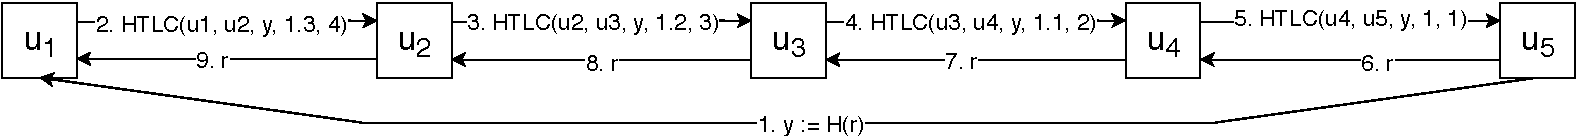
\includegraphics[width=\textwidth]{htlc-figure}
	\caption{An HTLC-based payment in the LN. The node $u_1$ pays $u_5$ using $u_2$, $u_3$ and $u_4$ as intermediaries. 
		Here we assume that each node charges a fee of $0.1$ and time is measured in days.\label{fig:htlc}}
\end{figure*}

\subsubsection*{Single channel updates}

An \textit{LN transaction} is an atomic update of one or multiple channels.
To send a payment to Bob, Alice negotiates a new channel state.
Each channel state is reflected in a \textit{commitment transaction} -- a bitcoin transaction that spends the funding transaction and distributes the funds to both parties in some proportion.
Outputs of commitment transactions are called \textit{Hash time-locked contracts}, or \textit{HTLC}s.
HTLC is defined by a Bitcoin script that gives the funds either to one party, if it provides a pre-image of a given hash, or to the other party after a timeout.
For instance, if Alice wants to send $x$ coins to Bob, she first asks him for a \textit{payment hash}.
Bob generates a random number $r$ and send its hash $H(r)$ to Alice in a message called an \textit{invoice}.
Alice then \textit{offers} Bob an HTLC that would give him $x$~coins if he provides a preimage of $H(r)$ before time $t$, or return the coins to Alice otherwise.
Bob must \textit{claim} the payment before time $t$.
If he provides $r$, the HTLC \textit{resolves}: the balances in the next commitment transaction outputs will reflect the new distribution of channel funds.
The other way for an HTLC to be resolved is timeout.
A payment channel can keep track of multiple unresolved HTLCs concurrently.

The cornerstone of LN security is its \textit{revocation} mechanism.
A channel partner may try to cheat by trying to close the channel with an earlier state.
In this case, the counterparty is guaranteed to get all funds from the channel if they react within a timeout.
The party that initiates the channel closure must wait until their portion of the funds becomes available.
For instance, if Alice initiates a channel closure, she must wait until her funds become available.
If the closure is a cheating attempt, Bob can dispute it before the timeout and take control of all channel funds.


\subsubsection*{Multi-channel updates}

Multi-path payments use onion routing to enforce the order of intermediary nodes.
Each HTLC is onion-encrypted so that each intermediary node only knows the immediate previous and next nodes, but not the final sender or receiver.
Transaction fees are collected by intermediary nodes as a difference between the amount in the HTLC they receive and the HTLC they send as part of the same transaction.
Note that if a payment fails, no fees are collected, as all pending balance updates roll back.

A multi-hop transaction leverages a path of channels between a sender and a receiver (who might not share a channel between them).
A transaction must ensure the atomicity of the transfer: either all balances along the path are updated or none of them are.
For that, the LN relies on Hash Time-Lock Contracts (HTLCs), 
excerpts from the Bitcoin's scripting language that 
permit a node ($u_1$) to lock $x$~coins in a channel between two nodes ($u_1$ and $u_2$) 
and release them according to the encoded conditions.
The terms for the HTLC($u_1, u_2, y, x, t$) are defined with a hash value $y := H(r)$, 
where $r$ is chosen uniformly at random, 
an amount $x$ of coins, and a timeout $t$, as follows: 
(i) If $u_2$ reveals a value $r$ such that $H(r) = y$ before $t$ expires, $u_1$ pays $x$ to $u_2$; 
(ii) if $t$ expires, $u_1$ receives $x$ back.

LN relies on HTLCs to enable multi-hop transactions. 
All HTLCs along the path use the same hash value $y=H(r)$ aiming to achieve atomicity expecting that 
none of the intermediate balances can be updated before the receiver reveals $r$, and all of them can be updated after that.
An illustrative example of an HTLC-based transaction is depicted in~\cref{fig:htlc}.
Here, the user $u_1$ transfers $1$ bitcoin to $u_5$ using $u_2$, $u_3$ and $u_4$ as intermediaries. 
For that, $u_5$ locally chooses a value $r$ 
uniformly at random, computes the cryptographic challenge for the HTLC as $y := H(r)$, 
and sends $y$ to the sender (step 1).
The message encoding $y$ is called an \textit{invoice}.
Then, the payment starts with a commit phase (steps 2-5) where every pair of nodes, 
starting from the sender, establishes an HTLC using $y$.
After the commit phase is finished, the transaction enters the release phase.
Here, the receiver reveals $r$ to $u_4$ to fulfill the contract (step 6), 
triggering thereby the release phase where every pair of nodes fulfills their 
contract from the receiver to the sender (steps 6-9).

It is important to note two aspects here.
First, every intermediary user charges a fee for the forwarding service provided. 
For instance, $u_2$ receives $1.3$~coins but only forwards $1.2$~coins, getting a fee of $0.1$~coins. 
Second, the time parameter of the contracts throughout the path is decreasing to ensure that no user loses coins. 
For instance, the HTLC between $u_1$ and $u_2$ sets a timeout of four days 
whereas the timeout in the HTLC between $u_2$ and $u_3$ is only three days.
This facilitates that 
$u_2$ has enough time to settle the contract with $u_1$ after receiving $r$ from $u_3$.
There is an inherent trade-off: channels with short timelocks open the risk of not being able to dispute a fraudulent transaction in case of blockchain congestion, and long timelocks open up a DoS vector, where an attacker can route many unsettled payments through a channel and effectively block it until the timelock expires.

\subsection{P2P network and routing}
LN is source routed.
Nodes exchange information about channels, and each node chooses routes based on the local view of the network graph.
The graph includes total channel capacities but not local balances of the counterparties.
Using HTLCs enables atomicity of channel updates in multi-path transactions.
For instance, Alice can pay Charlie via Bob by using the same hash value along the route.
If Charlie redeems the payment from Bob, then Bob can use the same pre-image to claim funds from Alice, otherwise no funds move.

LN nodes gossip about newly opened channels that are marked as available for routing.
Based on this information, each node maintains a local view of the network, and uses it to calculate routes to the receiver.
As total channel capacities are known, the sender only considers channels with the capacity larger than $X$ for a payment of amount $X$.
However, this is insufficient to prevent routing failures, because the distribution of funds in channels is not known.
The ability of channel parties to send or forward payments is limited by their \textit{local} channel balances.
Initially, if Alice opens a channel with Bob, all funds are on her side.
This means that she can send up to the total capacity, but she can not receive.
As the local balances change, the routing capabilities of the channels in both directions are also changing.

In case of payment failure, the sender is notified by an error message which channel has failed, and will presumably re-launch route generation function with the failed channel excluded.
This procedure repeats for a pre-set number of tries, or until a payment succeeds.
Given the external constraints it is sill not clear that a better approach than systematically probing for paths exist even though active research is being conducted in this area~\cite{Pickhardt2019a, Prihodko2016, Grunspan2018, Pickhardt2019, Piatkivskyi2018, Sivaraman2018, Bagaria2019, Roos2018}.

\subsection{Privacy}
Another aspect of LN relevant for this work is privacy.
Bitcoin is pseudonymous: while blockchain addresses are not linked to real world identity, and users are encouraged to not reuse them, the transaction graph can be extracted and analyzed.
In contrast, LN payments are only sent to a short chain of randomly chosen nodes along the route from a sender to a receiver.
Due to onion routing, each intermediary node only knows the previous and the next hops, but not the whole route and even not its position in the route.
This supports the presumption that Lightning payments provide more privacy than layer-one Bitcoin transactions.
However, our research as well as a probing attack described in~\cite{Dam2019} show that it is possible for an attacker to reveal balances of other channels of their channel partner.

\subsection{Implementations}
The development of the LN is guided by a set of request for comments (RFC) documents called "Basics of Lightning Technology" (BOLTs)~\cite{BOLT}, 
which are then followed by several implementation teams.
The three most advanced implementations available in 2020 are LND~\cite{LND} (implemented in go), c-lightning~\cite{clightning} (implemented in C), and Eclair~\cite{Eclair} (implemented in Scala).
Other implementations at earlier stages of development include
Electrum~\cite{ElectrumWebsite, ElectrumLightningAnnounce}, lit~\cite{lit}, lpd~\cite{lpd}, ptarmigan~\cite{ptarmigan}, and rust-lightning~\cite{rustlightning}.

Our results presented in~\cref{Chapter06LNprobing} have been obtained from the live network.
At the time of our experiments, the attack in question seemed to be relevant to all nodes regardless of the implementation.
Some of the countermeasures we propose can be implemented on the protocol level, and some on the implementation level.

Our research in~\cref{Chapter07LNattacks} and~\cref{Chapter08HTLClimit} is concerned with the definition of the LN as described in the BOLTs and thus the results apply equally to every implementation.


\section{Our contributions}
Our contributions in this part are threefold.

\paragraph{Discovering channel balances}
First, we study the privacy of LN balances.
The LN protocol provides no way for a node to know how funds are split in remote channels.
We ask the question: how private is this information in practice?
As it turns our, a low-resource attacker can infer balances of most of the channels using \textit{probing}.
Specifically, by sending an unsolicited fake payment and observing the resulting error, the attacker can infer the balances of channels along the route.
We show that this technique scales to the whole network and allows to probe channel balances in most channels with a high precision.
This part of our work raises a question: can we strike a better balance between balance privacy and routing efficiency?
At the moment, LN nodes cannot use balance information for routing, which leads to failed payments, but balances are extractable by an attacker anyway.
We propose multiple potential countermeasures, including just-in-time routing.
Evaluating them remains an exciting avenue for future work.

\paragraph{Quantitative analysis of privacy attacks}
Second, we perform an quantitative analysis of LN's resistance to three previously described attacks on privacy.
Privacy in payment networks is defined in terms of value privacy (the attacker does not know how much is sent) and relationship anonymity (the attacker does not know who is paying whom).
In the LN, an additional definition is added: a wormhole attack allows an adversary to steal fees from honest intermediaries and temporarily block their funds.
How much of a threat do these attacks present?
This depends on a multiple factors: for an attack to be successful, a payment must pass through a path partially controlled by the attacker.
For the three attacks, we estimate this probability based on a simulated network for an array of parameters.
Our findings suggest that LN, as of 2019, depends on highly connected and highly capitalized nodes: in case a relatively small proportion of such nodes are compromised, the attacker succeeds with a high probability.

\paragraph{Analysis of a concurrency-related throughput limitation}
Third, we describe a not so well-known peculiarity of the LN protocol concerned with concurrent payments.
Due to the size limitations on Bitcoin transactions, LN channels can handle up to a certain number of unresolved payments.
An attacker can send payment from one node to another, blocking the capacity of channels along the route and depleting their "slots".
This effect may be critical for micro-payment applications -- a use case LN was initially meant to solve.
We evaluate the effect this limitation has for various payment amounts and how it has changed over two years, based on LN historical data.

